\documentclass{beamer}
%
% Choose how your presentation looks.
%
% For more themes, color themes and font themes, see:
% http://deic.uab.es/~iblanes/beamer_gallery/index_by_theme.html
%
\mode<presentation>
{
  \usetheme{Boadilla}      % or try Darmstadt, Madrid, Warsaw, ...
  \usecolortheme{default} % or try albatross, beaver, crane, ...
  \usefonttheme{default}  % or try serif, structurebold, ...
  \setbeamertemplate{navigation symbols}{}
  \setbeamertemplate{caption}[numbered]
} 

\usepackage[english]{babel}
\usepackage[utf8x]{inputenc}
\usepackage{booktabs}
\usepackage{multirow}
\usepackage[scale=2]{ccicons}

%\AtBeginSection[]
%{
%  \begin{frame}<beamer>
%    \frametitle{Plan}
%    \tableofcontents[currentsection]
%  \end{frame}
%}
%\AtBeginSubsection[]
%{
%  \begin{frame}<beamer>
%    \frametitle{Plan}
%    \tableofcontents[currentsection, currentsubsection]
%  \end{frame}
%}

\title[Patent Mining]{Classifying Patent Based on their Semantic Content \\ An empirical exploration into patents text mining}
\author[Bergeaud, Potiron, Raimbault]{Antonin Bergeaud \and Yoann Potiron \and Juste Raimbault}
\institute[]{Banque de France, Keio University and ISC-PIF}
\date{November 2018}

\begin{document}

\begin{frame}
  \titlepage
\end{frame}

\section{Introduction}
\begin{frame}{Motivation}
    %Patenting is increasing, big data blablabla
    
    \textit{Patenting as a footprint of technology and its coevolution with science and culture~\cite{bais2010praise}}

\bigskip
\centering

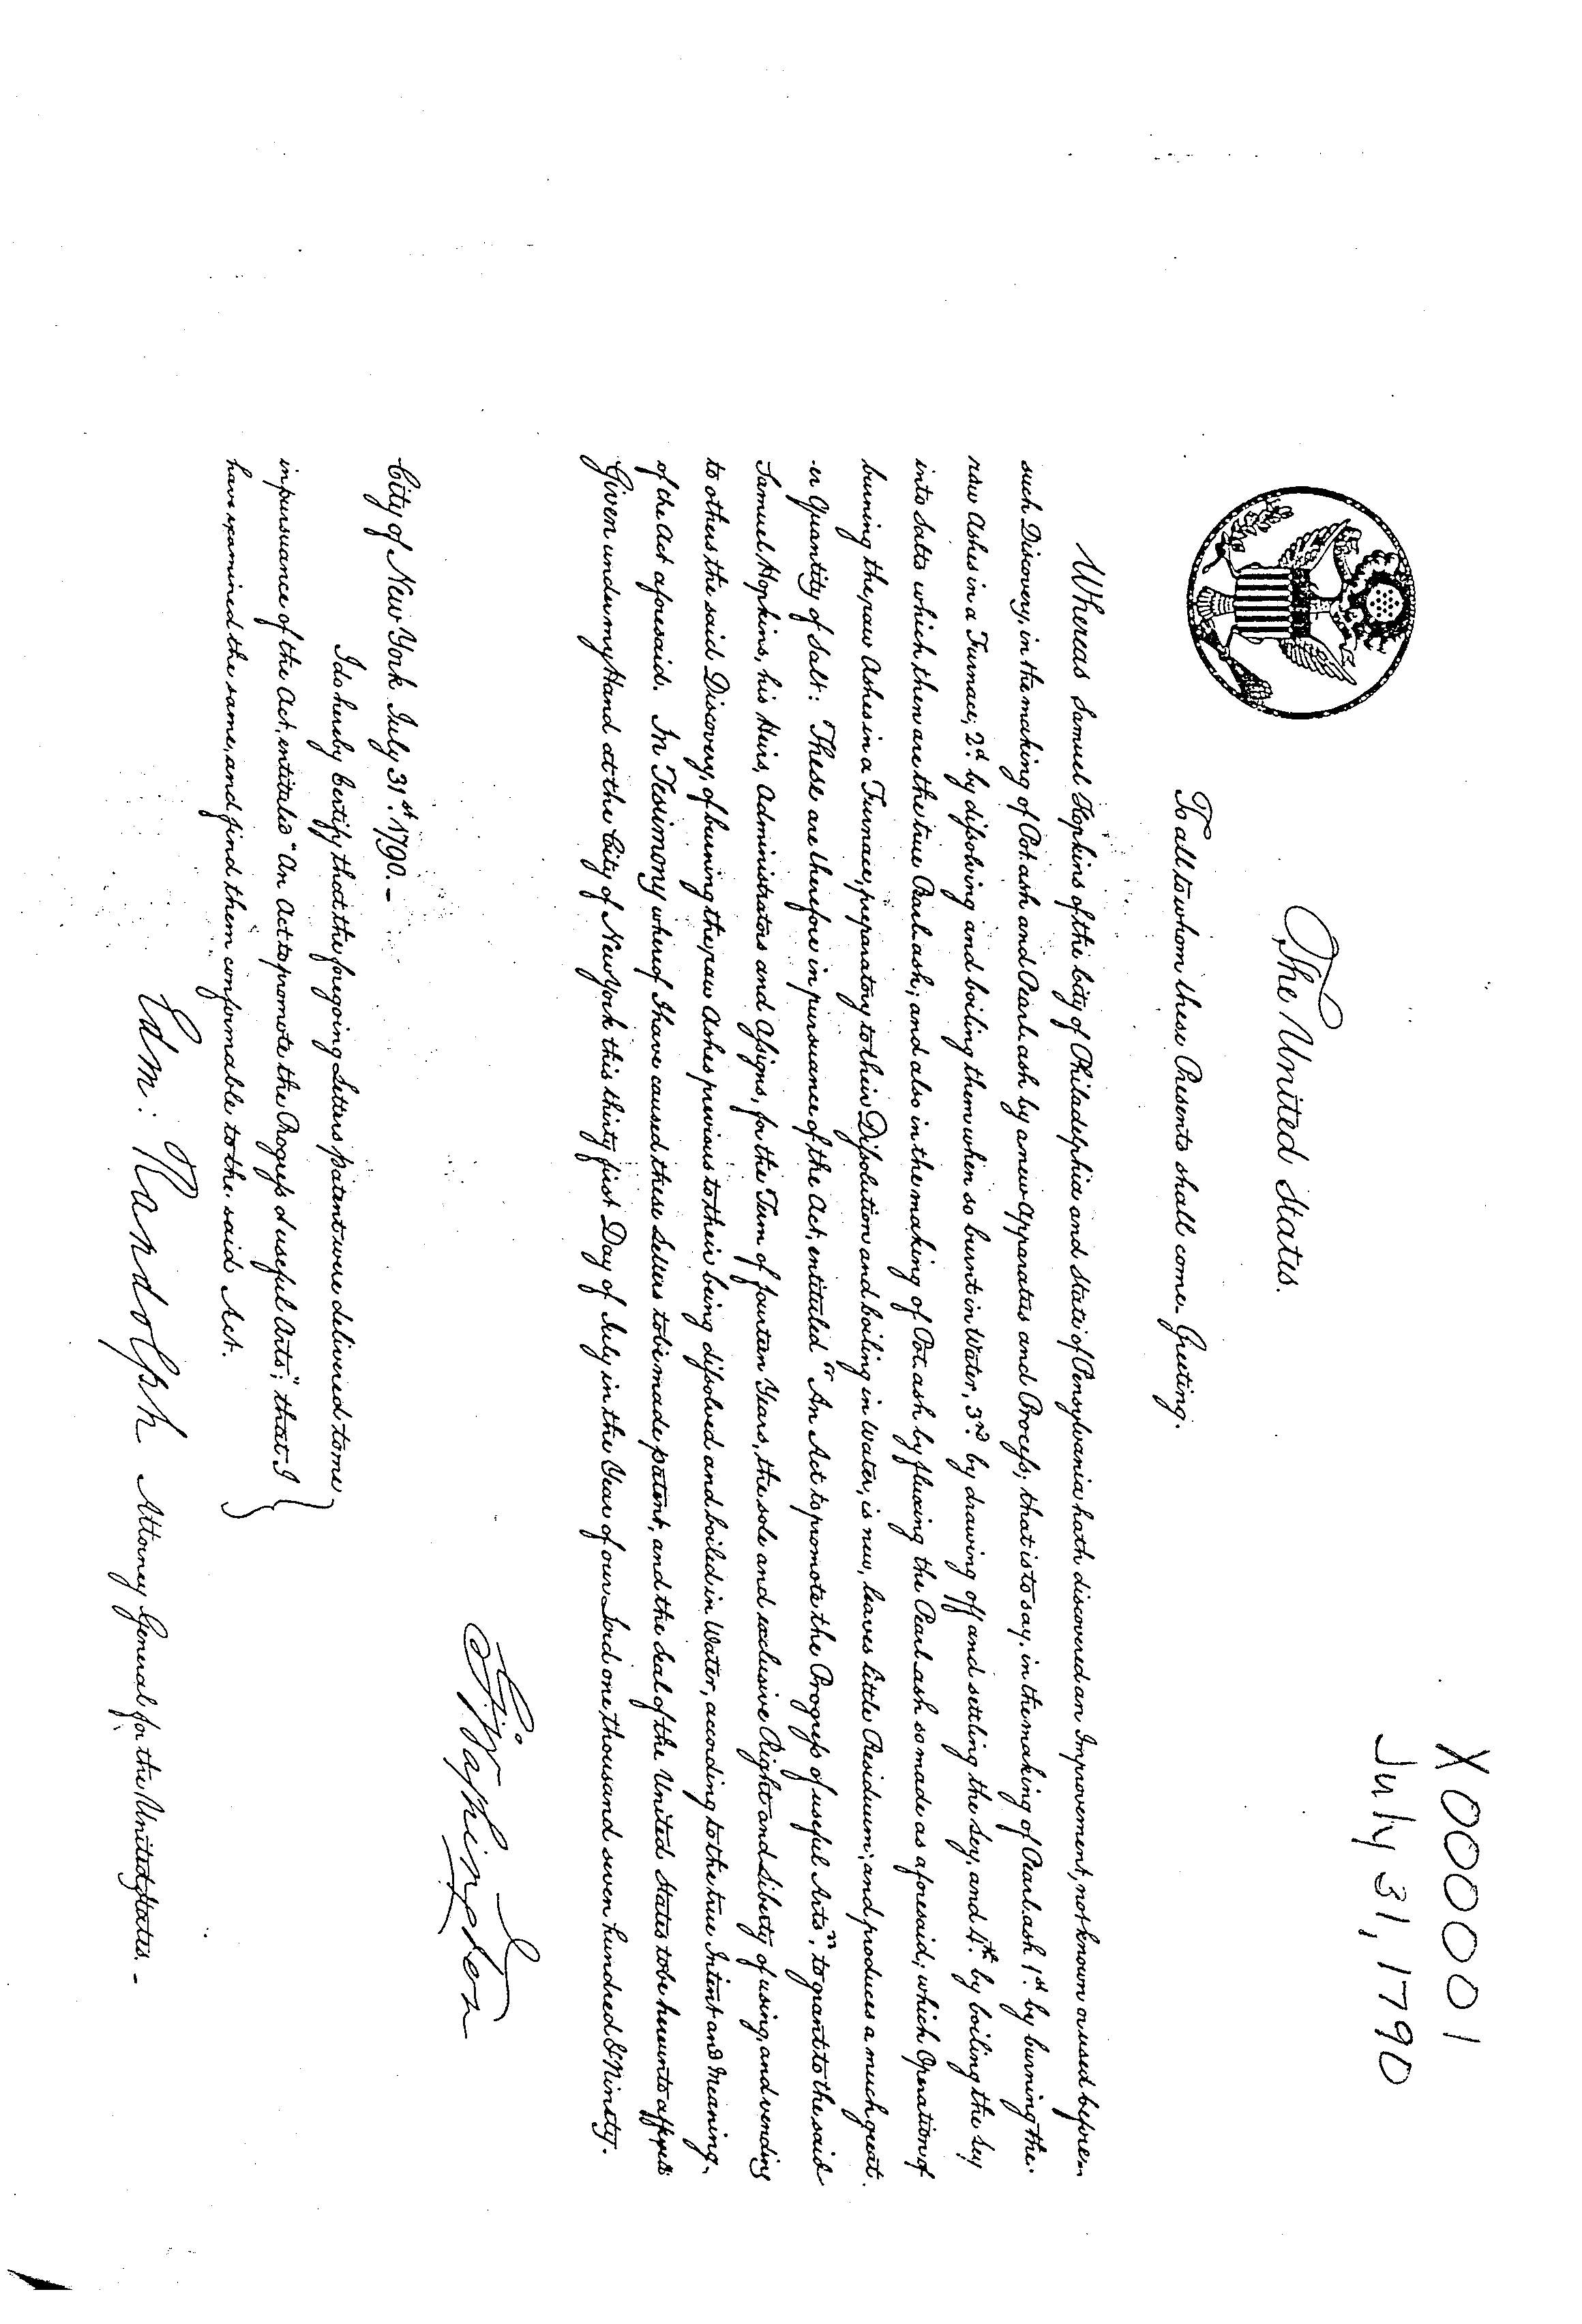
\includegraphics[width=0.35\textwidth,angle=90]{figures/USX1}
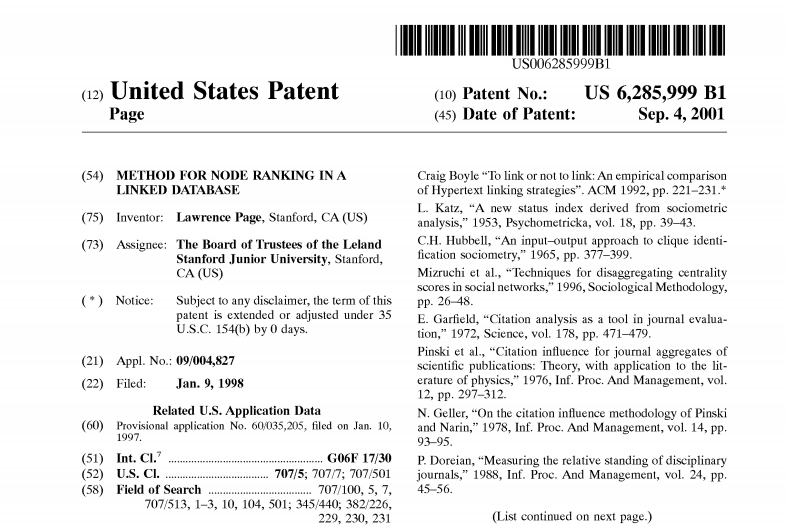
\includegraphics[width=0.45\textwidth]{figures/pageRank}
    
\end{frame}

\begin{frame}{Why study patents ?}
\justify

$\rightarrow$ Applied Epistemology : particular case of the ecology and evolution of knowledge ; propagation of knowledge

$\rightarrow$ Economics~\cite{griliches1998patent} : dynamics of innovation ; R{\&}D returns ; innovation at the core of endogenous growth theories~\cite{aghionhowitt1992}

\bigskip

\textbf{Examples :}

\begin{itemize}
\item \cite{Youn:2015fk} interaction between technological fields ; combinatorial nature of inventions
\item \cite{2016arXiv160207928B} citation network analysis to detect emerging research front
\item \cite{gerken2012new} \cite{tseng2007text} semantic analysis
\end{itemize} 

\end{frame}


%\begin{frame}{What we do}
%\end{frame}
\begin{frame}{A large scale semantic insight into USPTO database}
    
    % integrer le ``what we do'' ici ?   
    
    \textbf{Proposed approach}
    
    \textit{Complement existing patent office classifications using patent semantic content}
    
    \bigskip
    
    \textbf{Takeaway results}
    
    $\rightarrow$ \textit{An endogenous semantic classification is constructed for the full USPTO abstracts and titles, 1976-2012}
    
    \bigskip

    $\rightarrow$ \textit{Information carried is complementary to the technological classification}
    
    
\end{frame}
\section{Background}

\begin{frame}{Patent data}
    
    
\end{frame}
\begin{frame}{Descriptive statistics}
    % summary of our database ?
\end{frame}
    
\begin{frame}{Database construction}
    
Construction of a Database from US Patent and Trademark Office redbook 1976-2012 (full patent description), which provide raw data but on separate files and different formats

\bigskip

\textbf{Data Collection Procedure}

\begin{itemize}
\item Automatic download of raw data file
\item Parsing depending on format : \texttt{dat} or \texttt{xml} (varying schema)
\item Uniformisation and storing in MongoDB
\end{itemize}

\bigskip

$\rightarrow$ 4391272 patents with text data ; dated by application date (current state of knowledge)

\end{frame}
\section{Methods}
\begin{frame}{Extracting relevant n-grams}
    
    % Situate regarding other classical approaches : LDA etc
    
    \textit{Text-mining in python with \texttt{nltk}~\cite{bird2006nltk}}, method adapted from
\cite{chavalarias2013phylomemetic}. Advantage over LDA: scalability and flexibility

   

\bigskip

\begin{itemize}
\item Parsing and tokenizing / pos-tagging (word functions) / stemming  with \texttt{nltk}
\item Selection of potential \textit{n-grams} (with $1 \leq n \leq 3$) with the rule $\bigcap \{NN \cup VBG \cup JJ \}$
\item Database insertion for instantaneous use (several days $\rightarrow$ 1min)
\item Estimation of \textit{n-grams} relevance, following co-occurrences statistical distribution (\textit{termhood} score as chi-2 score)
\end{itemize}
\end{frame}

\begin{frame}{Estimation of n-gram relevance}
    
    \begin{itemize}
        \item Termhood-based selection of a fixed number of keywords
        \item Estimation on temporal moving windows
        \item Filtering of network edge, with an additional exogenous control by technological class keyword concentration to filter nodes
    \end{itemize}
    
\end{frame}

\section{Results}
\begin{frame}{Optimizing network structure}
    
    \centering
    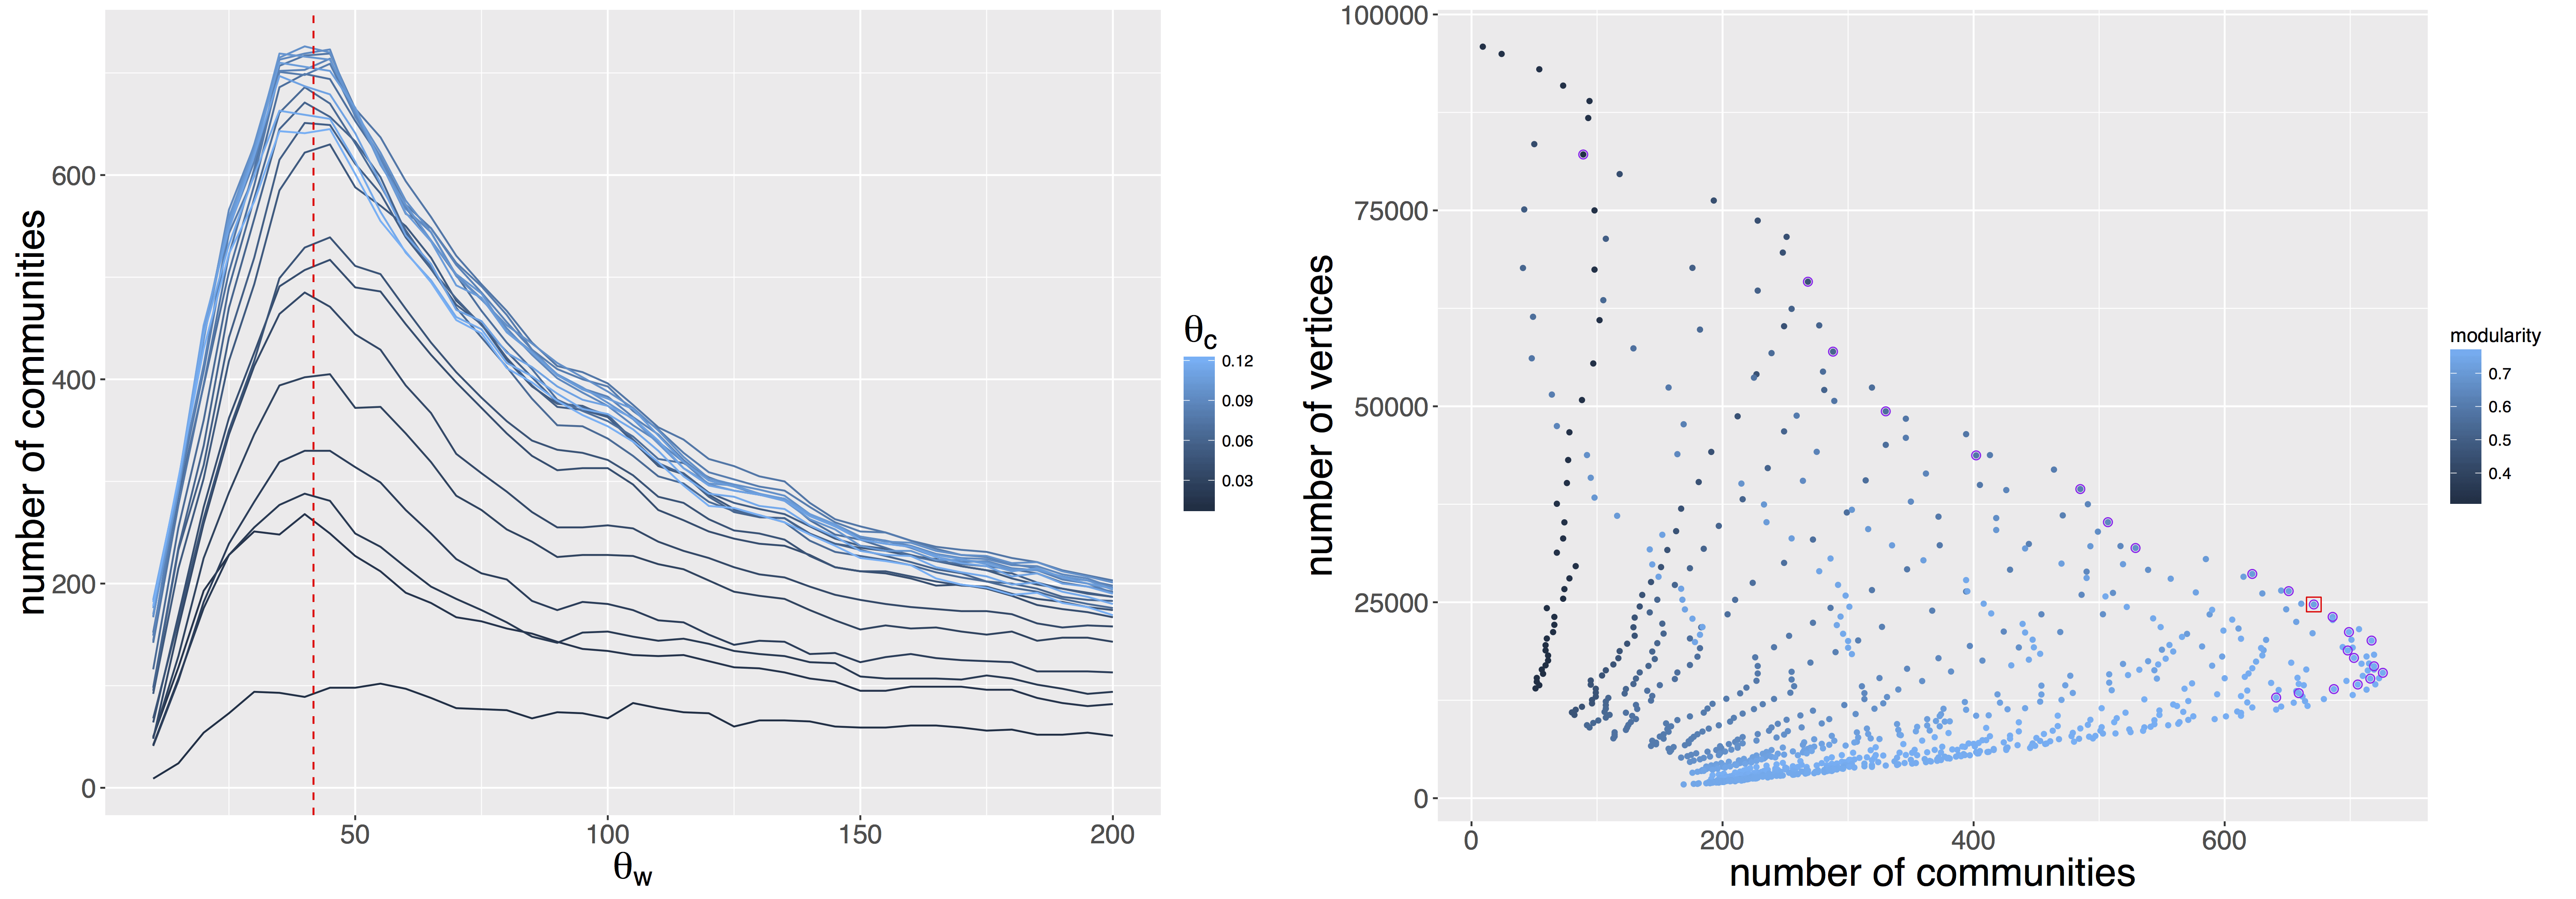
\includegraphics[width=\textwidth]{figures/Fig1.png}
    
    \medskip
    
    \textit{Pareto optimization on cutoff parameters for modularity, size and number of communities}
    
\end{frame}

\begin{frame}{Semantic network visualization}
   \centering
    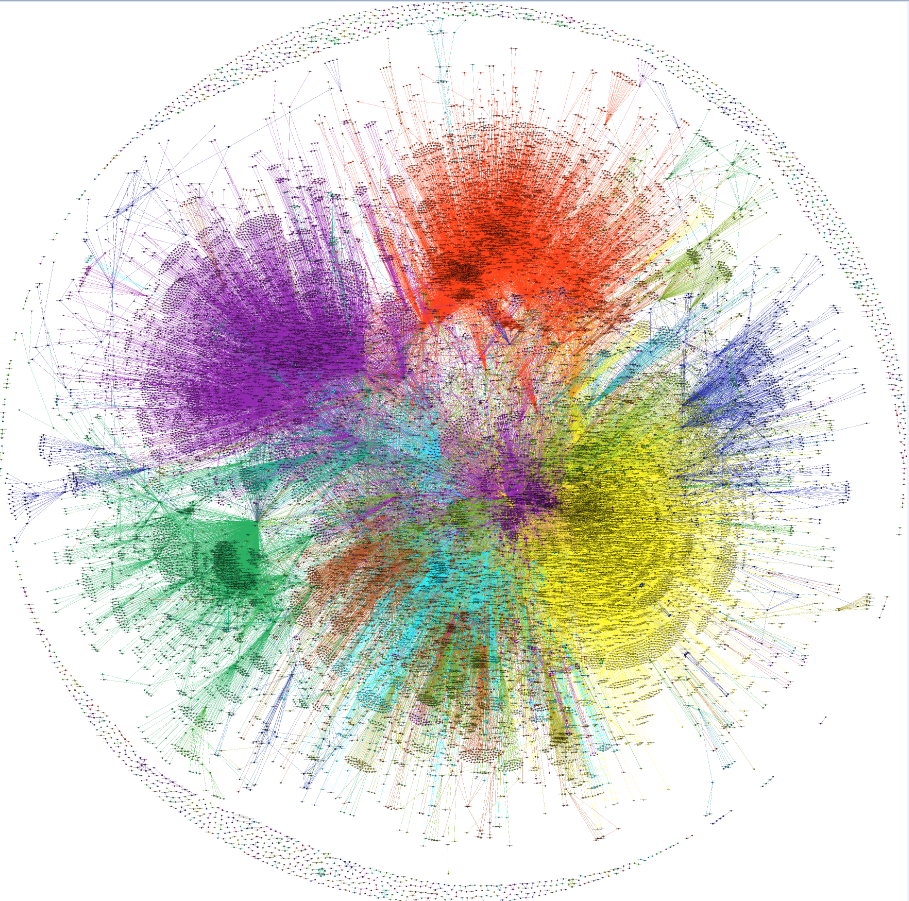
\includegraphics[height=\textheight]{figures/Fig2.png}
    
\end{frame}


\begin{frame}{Classes Examples (2000-2004)}

\justify

\begin{itemize}
\item Memory devices : \texttt{semiconductor memori devic; memori cell plural; memori cell transistor; layer ferroelectr}
\item Chemical analysis : \texttt{time-of-flight mass spectromet; chromatograph column; ion trap mass}
\item Particular steel : \texttt{martensit; austenit stainless steel}
\item Laser : \texttt{emit laser beam; vertic caviti surfac; vcsel}
\item Sewing : \texttt{circular knit machin; stitch; sew machin; embroideri}
\item Lithography : \texttt{lithograph mask; project beam radiat; heat-sensit; planograph print plate}
\item Tobacco : \texttt{cigarett filter; cigarett pack; tobacco; tobacco rod}
\end{itemize}
\end{frame}



\begin{frame}{Size of classes}
   \centering
    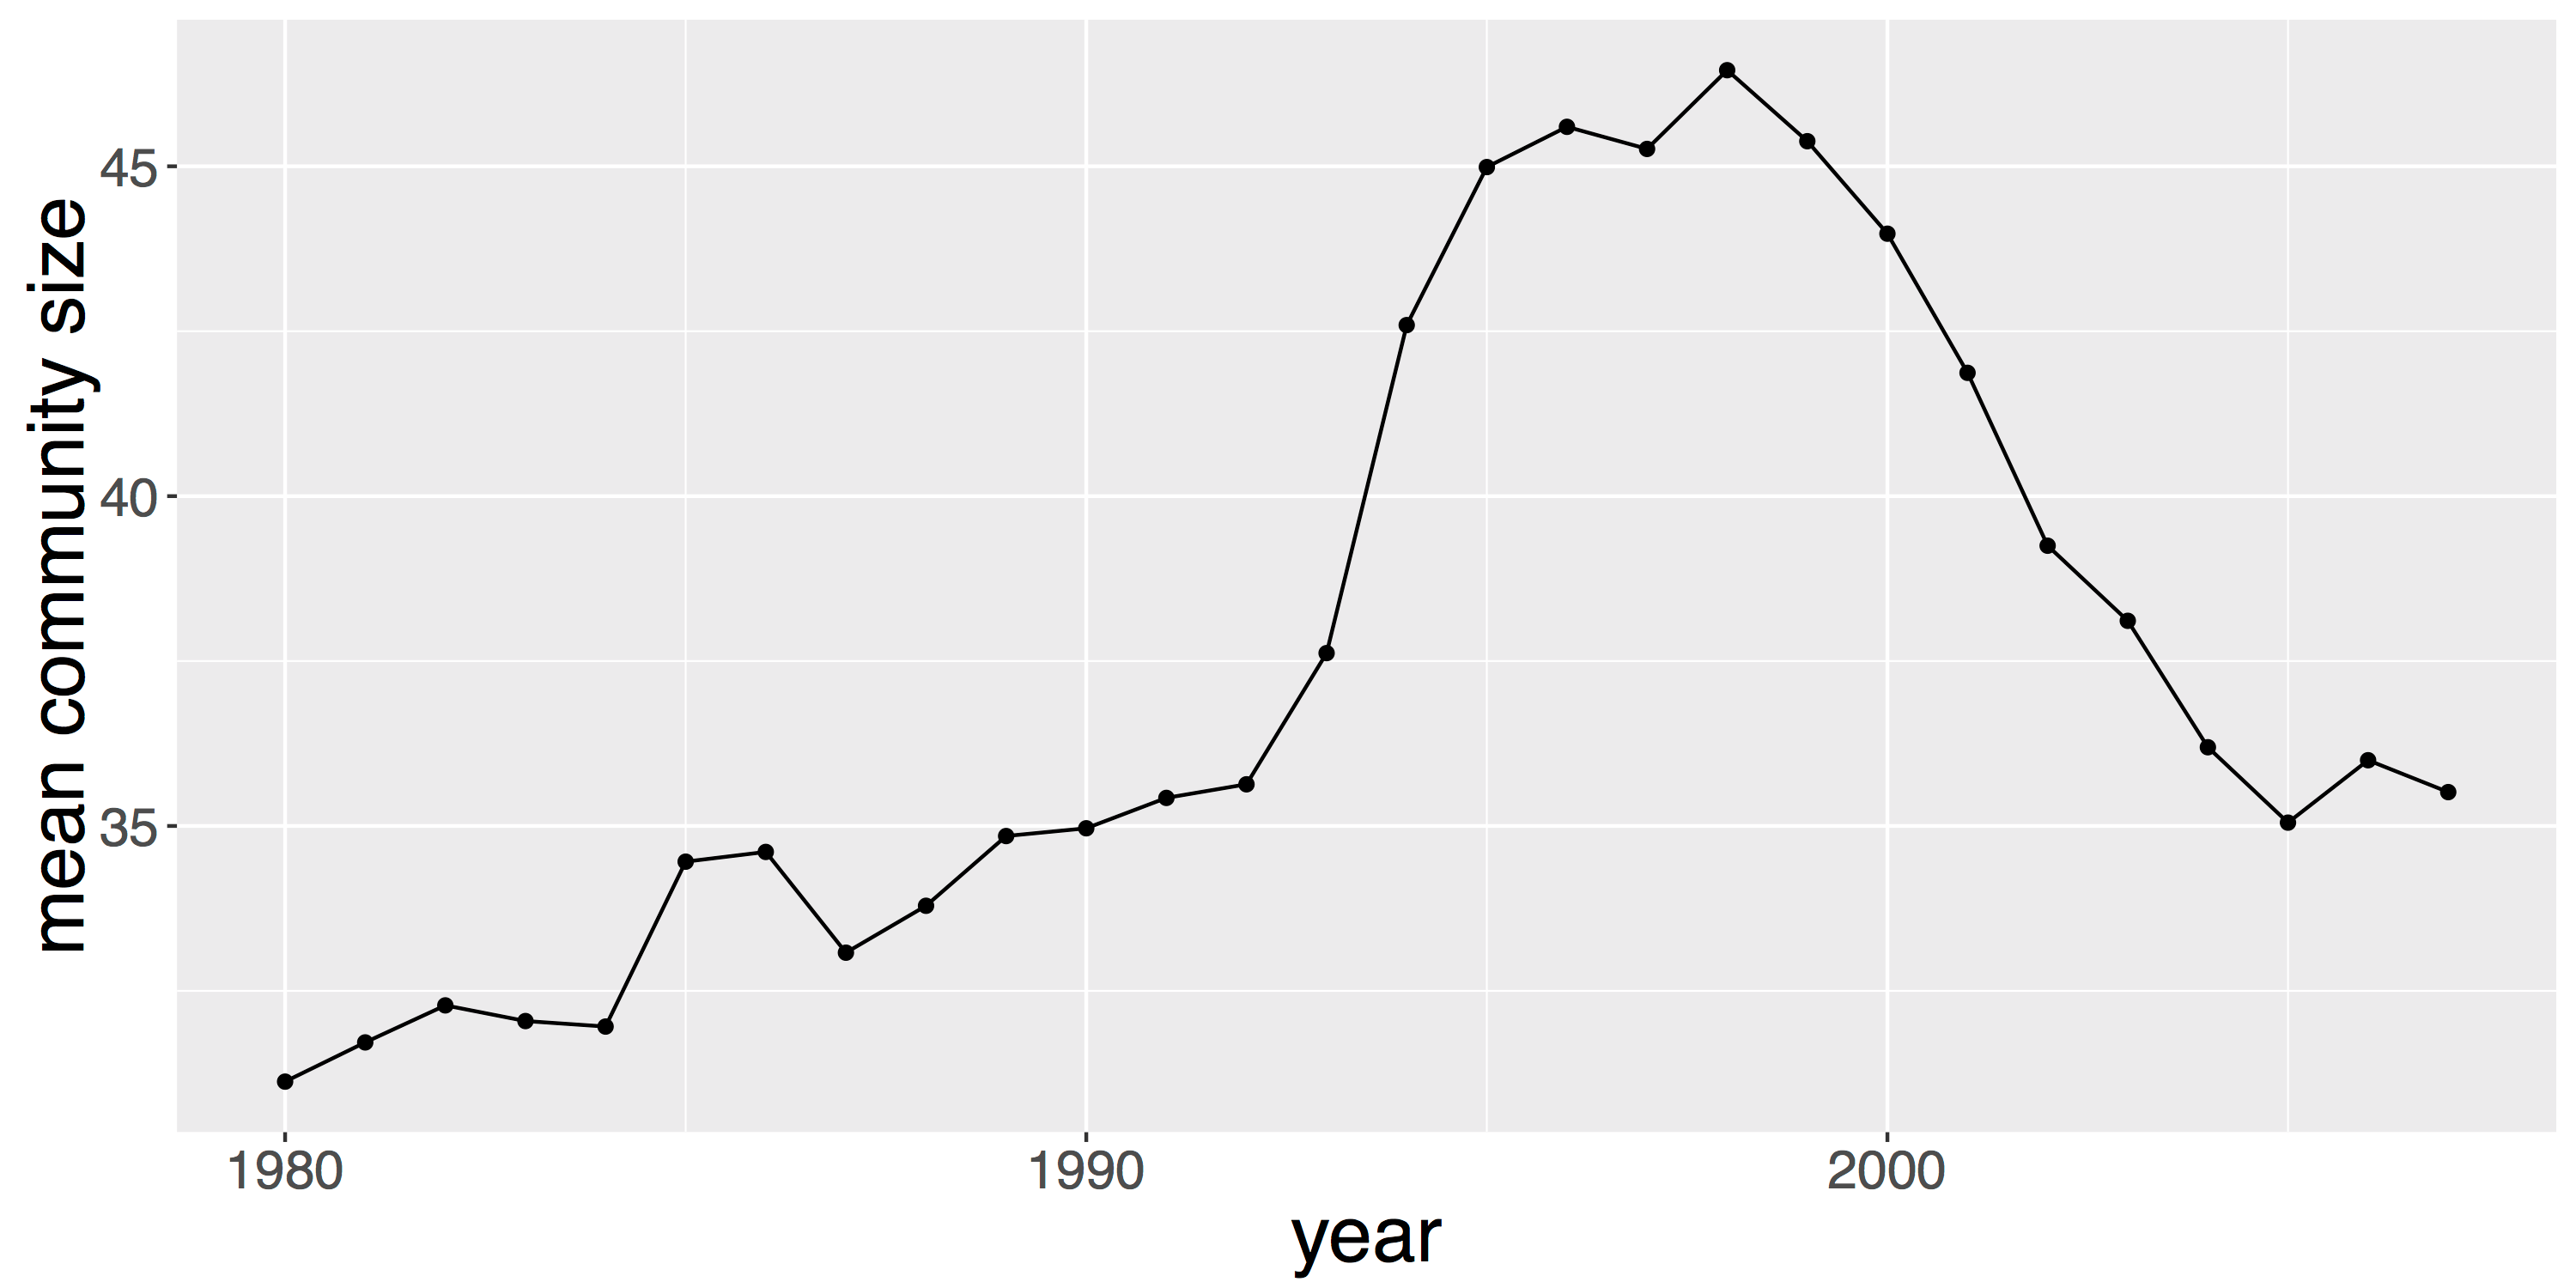
\includegraphics[width=\textwidth]{figures/Fig3.png}
    
    \medskip
    
    \textit{A peak in average class size around 1998}
    
\end{frame}

\begin{frame}{Hierarchical class structure}
   \centering
    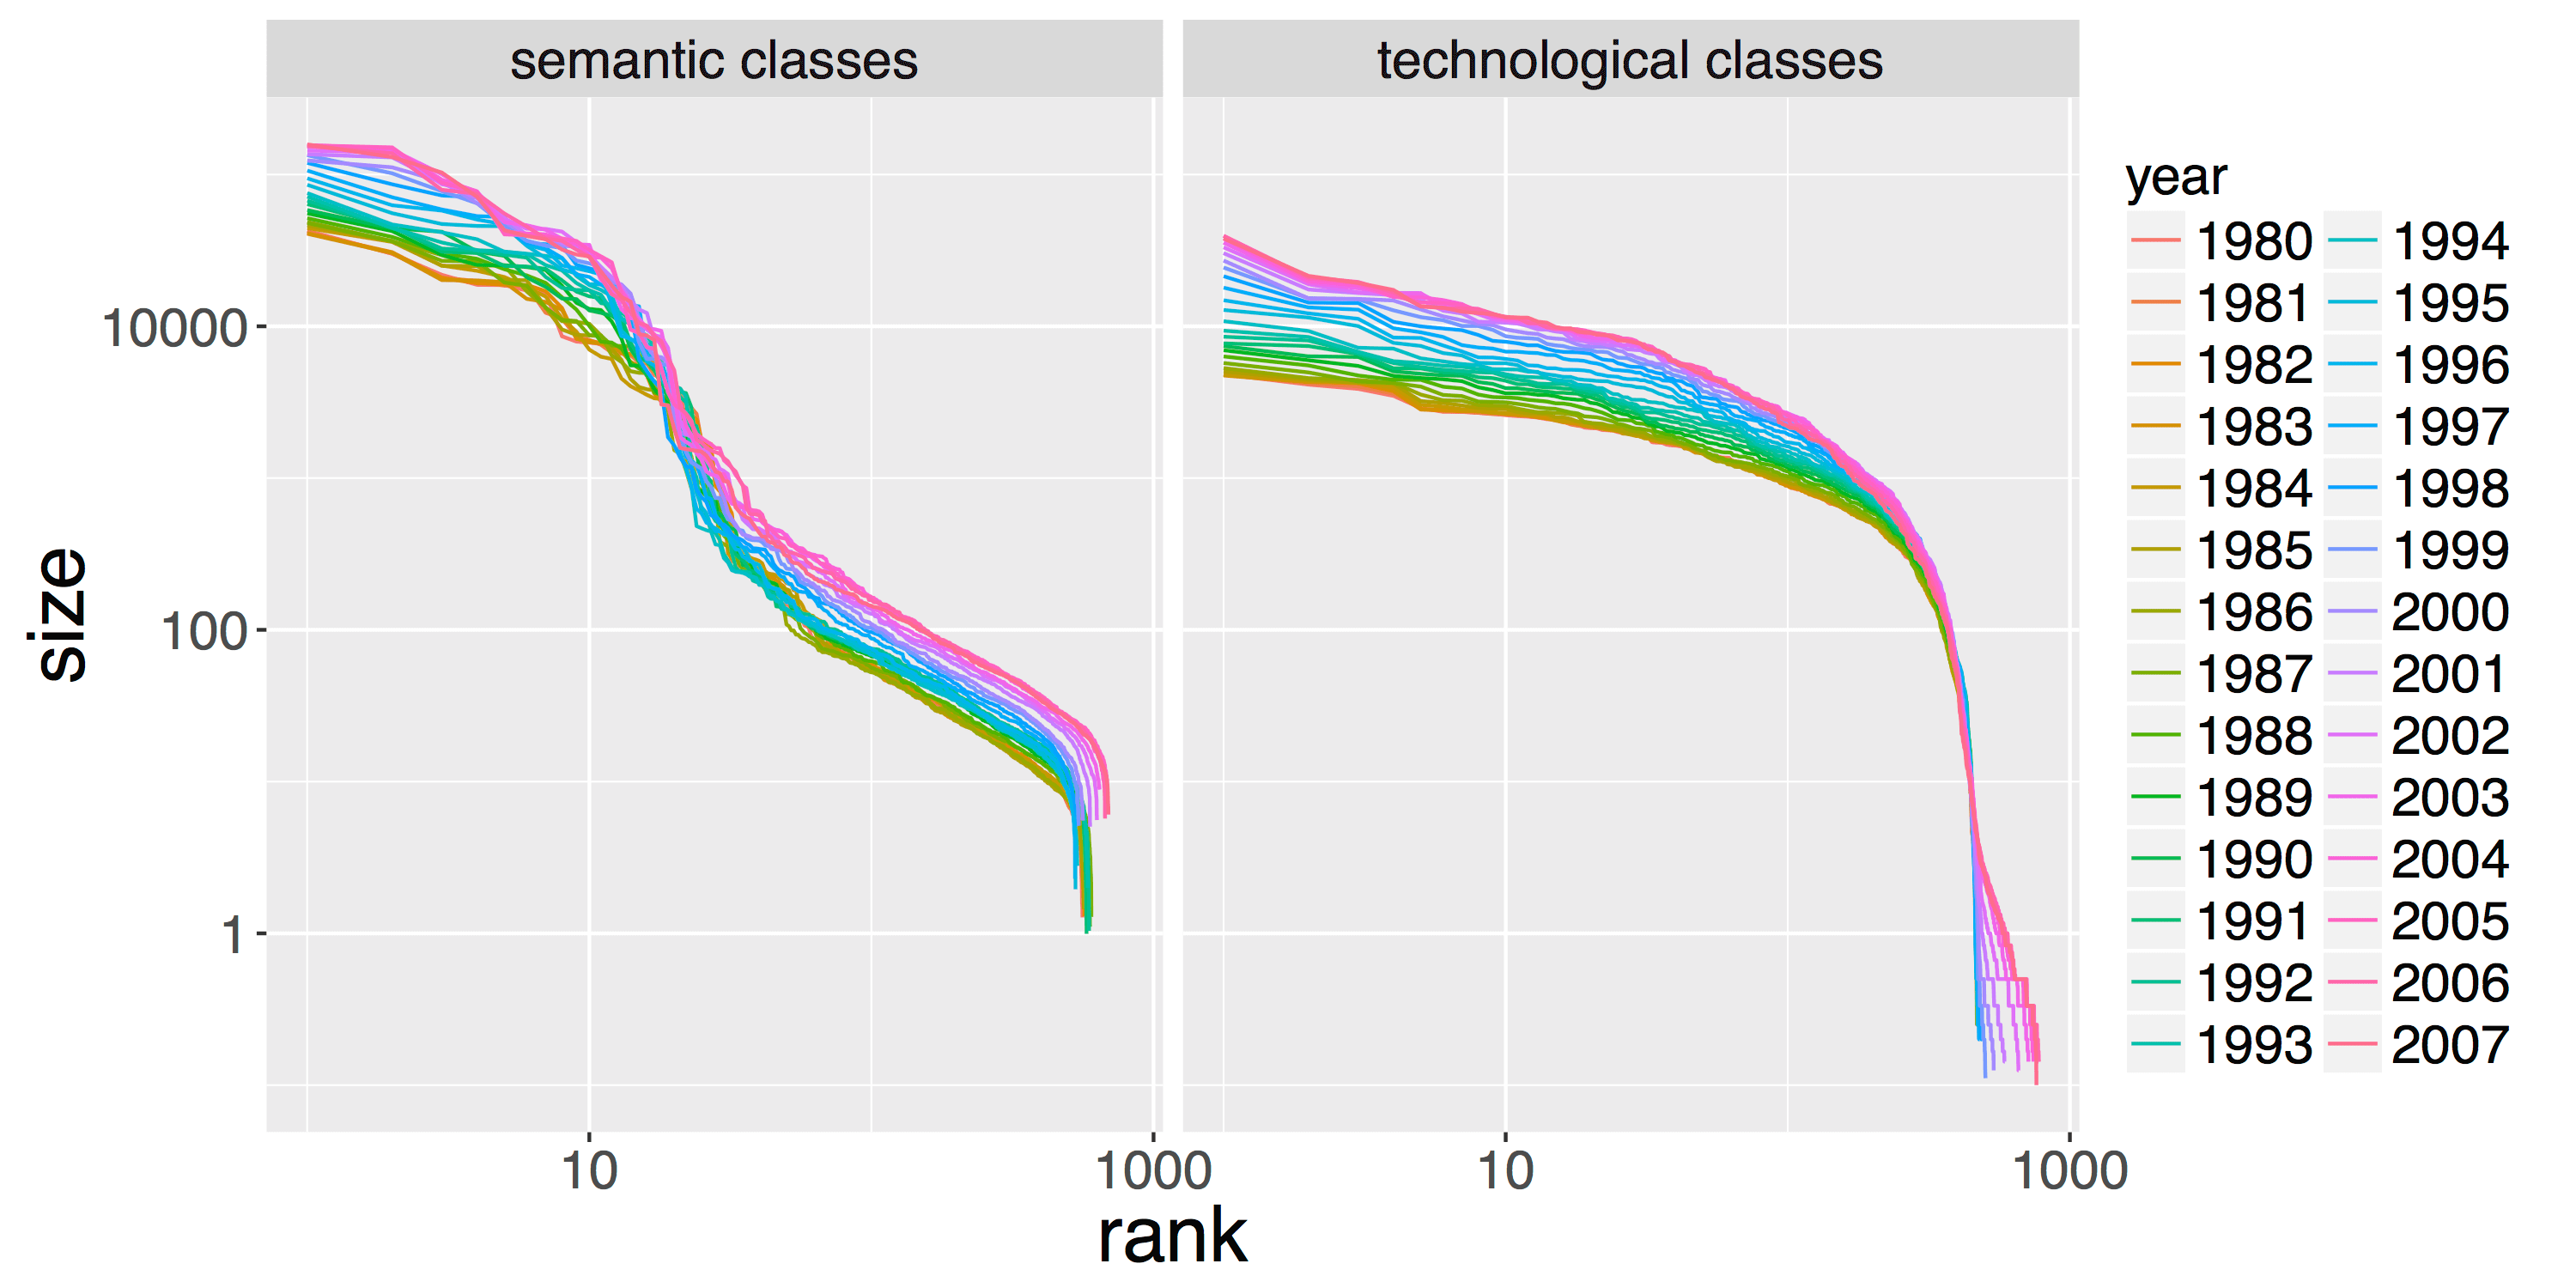
\includegraphics[width=\textwidth]{figures/Fig4.png}
    
    \medskip

    \textit{Fat-tail distribution of class size for both classification, closer to a power-law for semantic classes}
    
\end{frame}

\begin{frame}{Evolution of patent diversities}
   \centering
    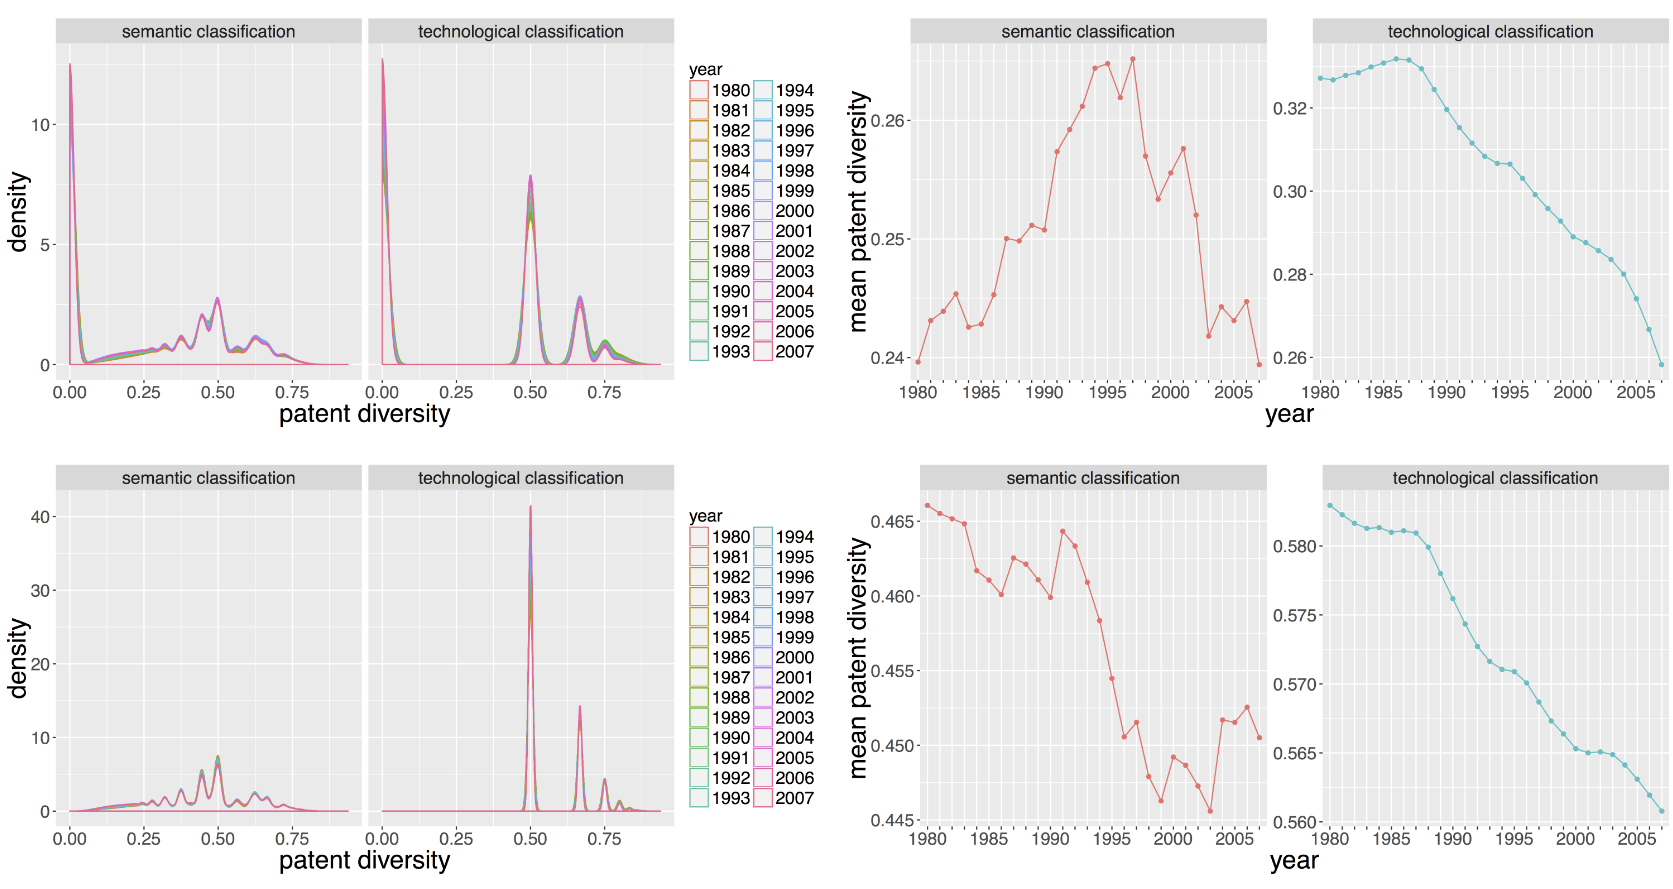
\includegraphics[width=\textwidth]{figures/Fig5.png}
    
    \medskip

    \textit{General increase in average invention specialization seen both for semantic and technological; semantic regime shift in 1996} 
    % "change in the regime of specialization, the new regime being caused by more single-class patents"
    
\end{frame}

\begin{frame}{Originality and generality measures}
   \centering
    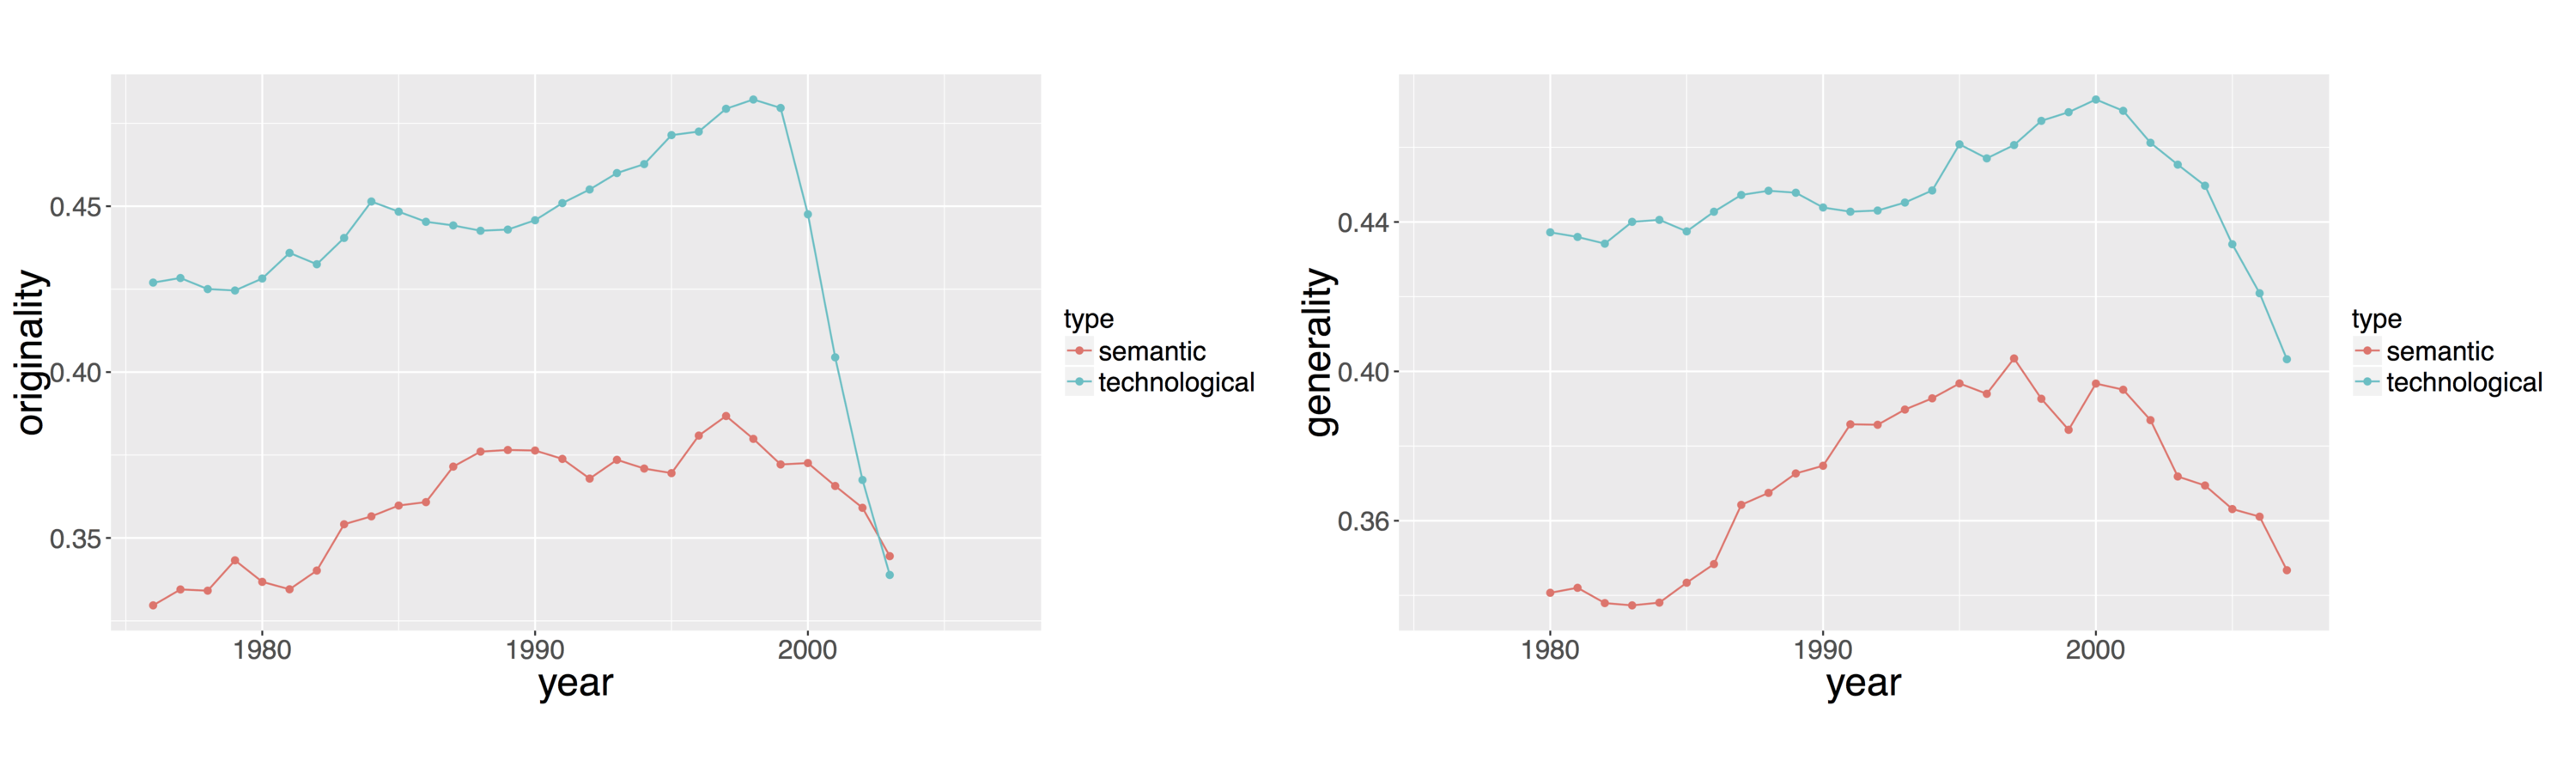
\includegraphics[width=\textwidth]{figures/Fig6.png}
    
    \medskip
    
    \textit{Systematically lower originality and generality (citation-based measures) for the semantic classification (consistent with the higher modularity shown therafter)}
    
\end{frame}

\begin{frame}{Interaction between classes: intra-classification overlaps}
   \centering
    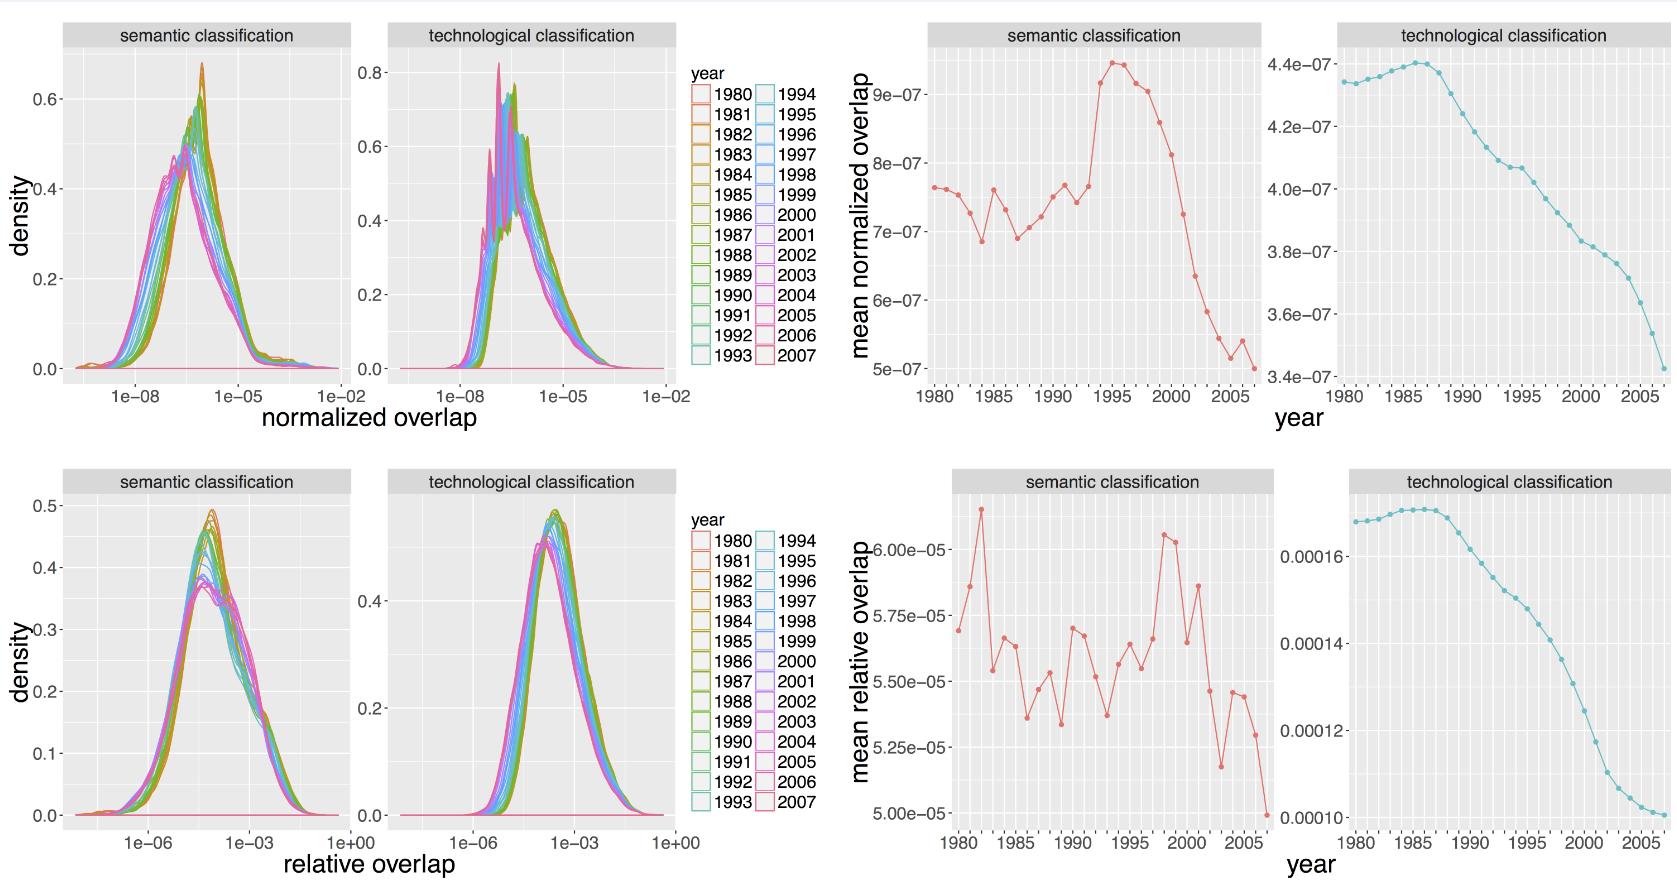
\includegraphics[width=\textwidth]{figures/Fig7.png}
    
    \medskip

    % techno : increasing specializatino trend
    % semantic : consistent with 1996 breakpoint in the structure of technologies - rq : how to control specifically that it is not an artifact of the method / or biased by sizes ?
    
    \textit{Increased technological specialization; qualitative regime shift confirmed in 1996 for the semantic classification}
    
\end{frame}

\begin{frame}{Inter-classification overlaps}
   \centering
    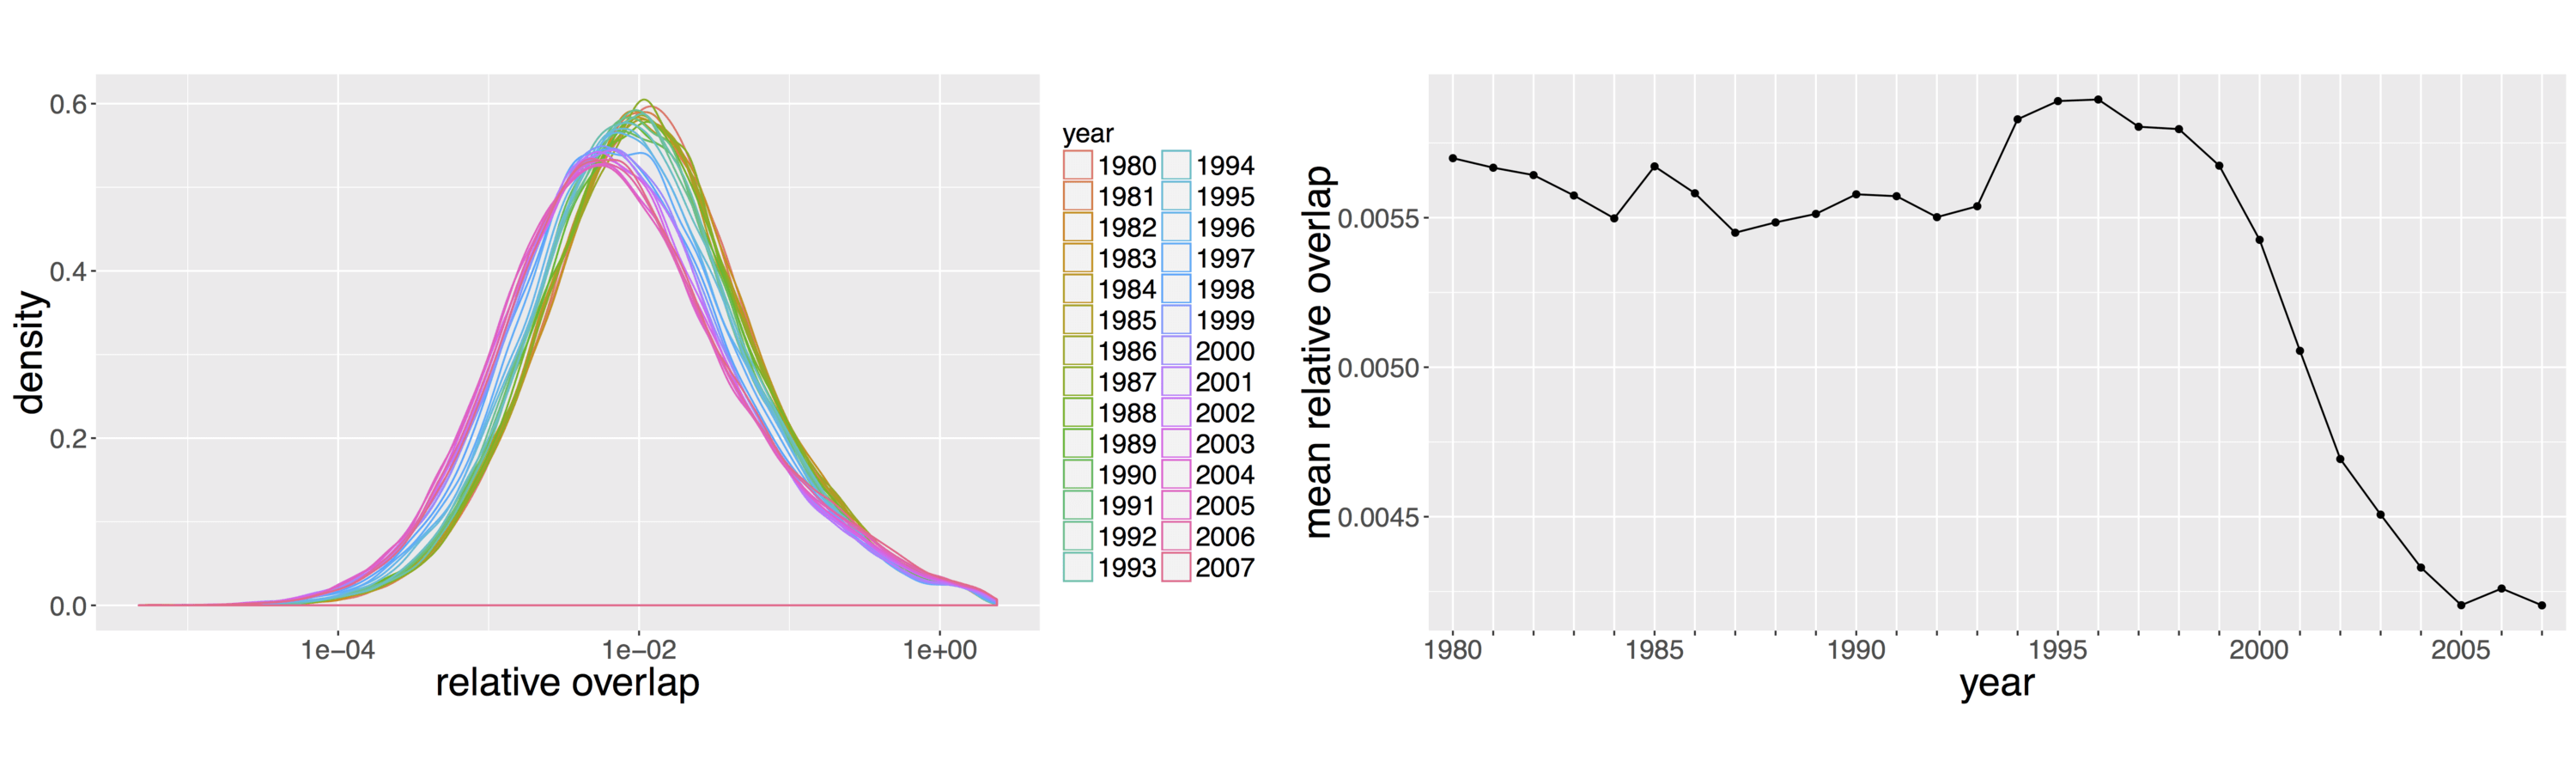
\includegraphics[width=\textwidth]{figures/Fig8.png}
    
    \medskip

    \textit{Confirms the change in nature of inventions around 1996} 
    
\end{frame}

\begin{frame}{Modularity of classifications}
   \centering
    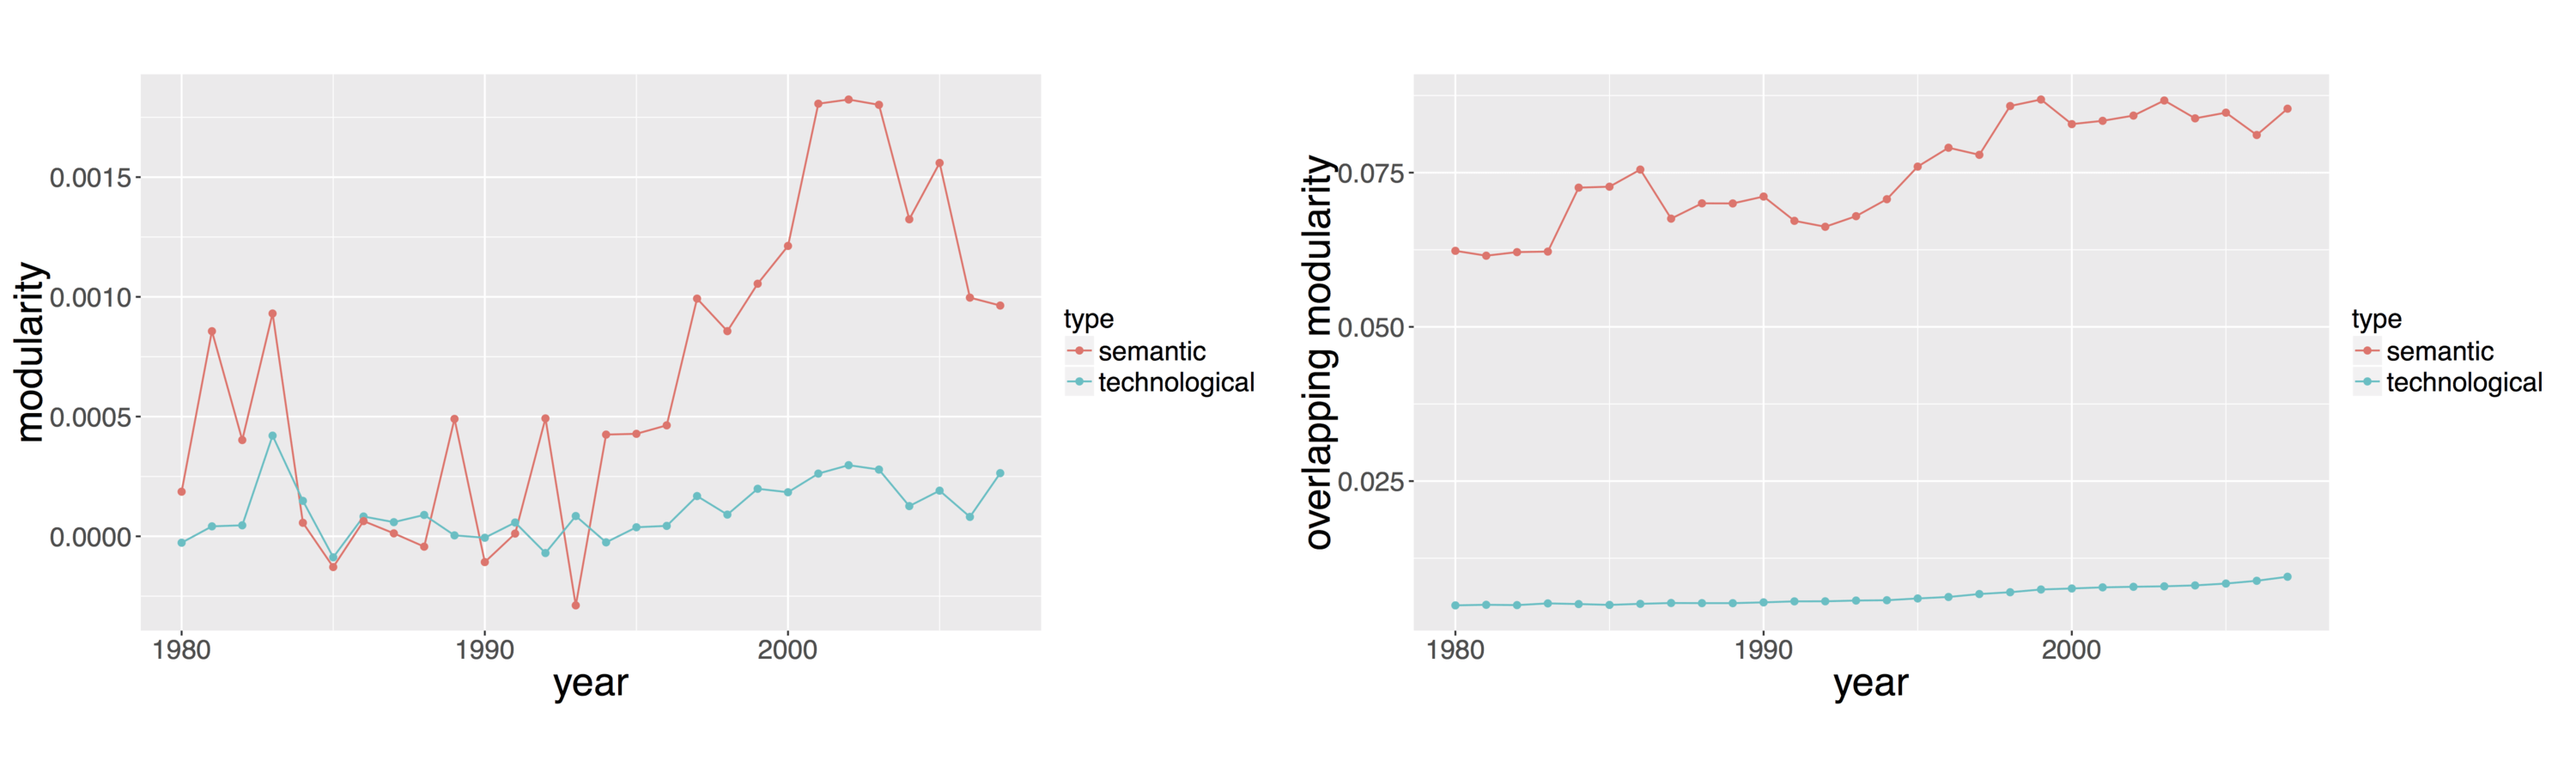
\includegraphics[width=\textwidth]{figures/Fig9.png}
    
    \medskip
    
    \textit{Semantic classification is more significant regarding the structure of the citation network, both for single-class and multi-class modularities.}
    
\end{frame}

%\begin{frame}{Stochastic Block Modeling to evaluate consistency of classifications}
    
    % tableau trop long, impossible a inserer
    
%\end{frame}


\section{Conclusion}

\begin{frame}{Discussion}
    \justify

    \textbf{Implications}
     
     \smallskip

    $\rightarrow$ Possible application to detection of emerging research fronts

    \smallskip
    
    $\rightarrow$ An interactive exploration of semantic content ?

    \textbf{Developments (ongoing)}
     
      \smallskip
     
     $\rightarrow$ Application on the European patent database
     
     \smallskip
     
     $\rightarrow$ Quantifying the diffusion of innovation in urban systems, and its co-evolution with the socio-economic structure
     
     \smallskip
     
     \textbf{Possible developments}
     
      \smallskip
     
     $\rightarrow$ Agent-based modeling of interactions between technologies
     
     \smallskip
     
     $\rightarrow$ Full-text mining and history of technology
     
    


\end{frame}

\begin{frame}{Conclusion}



\bigskip

\textbf{Open repository} at \texttt{https://github.com/JusteRaimbault/PatentsMining}\\\smallskip
\textbf{Raw database} at \texttt{http://dx.doi.org/10.7910/DVN/BW3ACK} and \textbf{Semantic classification database} at  \texttt{http:// dx.doi.org/10.7910/DVN/ZULMOY}\\\smallskip
\textbf{Acknowledgments}: thanks to ISC-PIF for access to the computation infrastructure.

\end{frame}




%%%%%%%%%%%%%%%%%%%%%
\begin{frame}[allowframebreaks]
\frametitle{References}
\bibliographystyle{apalike}
\bibliography{patents}
\end{frame}
%%%%%%%%%%%%%%%%%%%%%%%%%%%%



\end{document}